\documentclass{ctexart}
\usepackage{geometry}
\usepackage[dvipsnames,svgnames]{xcolor}
\usepackage{framed}
\usepackage{enumerate}
\usepackage{amsmath,amsthm,amssymb}
\usepackage{enumitem}
\usepackage{template}
\usepackage{tikz}

\allowdisplaybreaks
\geometry{left=2cm, right=2cm, top=2.5cm, bottom=2.5cm}

\begin{document}\pagestyle{empty}
\begin{center}\large
    极坐标下的图形面积
\end{center}
熟知极坐标系$(r,\theta)$中曲线$\rho(\theta)$从极角$\alpha$到$\beta$的面积为
$$A=\dfrac{1}{2}\int_a^b\rho^2(\theta)\di\theta$$
\begin{center}
    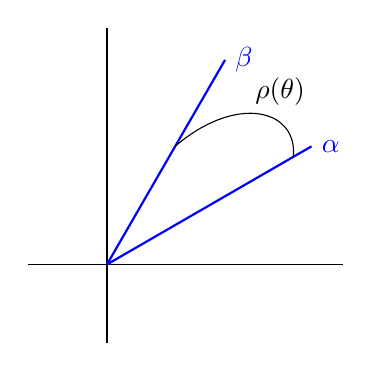
\begin{tikzpicture}
        \draw (-1,0)--(3,0);
        \draw (0,-1)--(0,3);
        \draw[line width =0.8pt,blue] (0,0)--(1.5,2.598) node[right]{$\beta$};
        \draw[line width =0.8pt,blue] (0,0)--(2.598,1.5) node[right]{$\alpha$};
        \draw[domain=30:60,samples=100] plot (\x:{sin(\x*3)+2*sin(\x*2)});
        \node at (2.2,2.2) {$\rho(\theta)$};
    \end{tikzpicture}
\end{center}
现在我们来看一些相关的问题.
\begin{problem}[Problem 1.]
    求极坐标系中三叶玫瑰线$r(\theta)=\sin(3\theta),0\leqslant\theta\leqslant 2\pi$所围成图形的面积.
\end{problem}
\begin{analyze}[Analysis.]
    我们也许会想到直接套用公式,即
    $$\begin{aligned}
        S
        &= \dfrac{1}{2}\int_{0}^{2\pi}\sin^2(3\theta)\di\theta \\
        &= \dfrac{1}{6}\int_{0}^{6\pi}\sin^2\varphi\di\varphi \\
        &= \dfrac{1}{6}\int_{0}^{6\pi}\dfrac{1-\cos2\varphi}{2}\di\varphi \\
        &= \dfrac{1}{6}\left.\left(\dfrac{\varphi}{2}-\dfrac{\sin2\varphi}{4}\right)\right|_0^{6\pi} \\
        &= \dfrac{\pi}{2}
    \end{aligned}$$
    然而查阅答案可知$S=\dfrac{\pi}{4}$.\\
    欸,问题出在哪里呢?\\
    我们仔细观察一下这个曲线在$\left[0,\dfrac{\pi}{3}\right]$和$\left[\dfrac{\pi}{3},\dfrac{2\pi}{3}\right]$的图像,分别用红色和蓝色标出.
    \begin{center}
        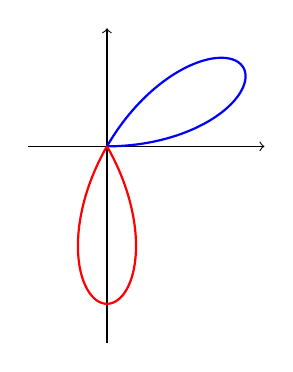
\begin{tikzpicture}
            \draw[->] (-1,0)--(2,0);
            \draw[->] (0,-2.5)--(0,1.5);
            \draw[line width =0.8pt,blue,domain=0:60,samples=100] plot (\x:{2*sin(\x*3)});
            \draw[line width =0.8pt,red,domain=60:120,samples=100] plot (\x:{2*sin(\x*3)});
        \end{tikzpicture}
    \end{center}
    我们再来看一下该曲线在$\left[\dfrac{4\pi}{3},\dfrac{5\pi}{3}\right]$的图像:
    \begin{center}
        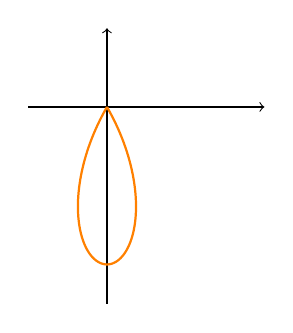
\begin{tikzpicture}
            \draw[->] (-1,0)--(2,0);
            \draw[->] (0,-2.5)--(0,1);
            \draw[line width =0.8pt,orange,domain=240:300,samples=100] plot (\x:{2*sin(\x*3)});
        \end{tikzpicture}
    \end{center}
    可以注意到,我们计算面积时将红色的部分和绿色的部分都计算了一遍,于是得到了不正确的结果.\\
    这是因为当$n$为奇数时,$r(\theta)=\sin(m\theta)$在$\theta\in\left[\dfrac{k\pi}{n},\dfrac{(k+1)\pi}{n}\right]$和$\theta\in\left[\dfrac{k\pi}{n}+\pi,\dfrac{(k+1)\pi}{n}+\pi\right]$时有
    $$r(\theta+\pi)=\sin\left(n\theta+n\pi\right)=-\sin{n\theta}=-r(\theta)$$
    极角相差$\pi$,极径取值也为相反数,在图像上的表现就是曲线的重合.因此我们在$[0,2\pi]$上的积分将重复计算该部分的面积,对于其它几片“叶”也是相同的.\\
    而当$n$为偶数时,又将得到不同的结果.请看$n=4$时的图像.
    \begin{center}
        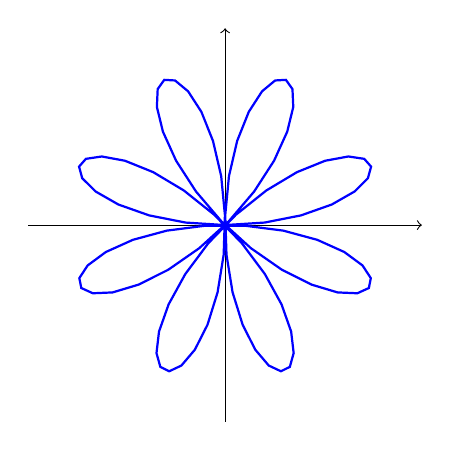
\begin{tikzpicture}
            \draw[->] (-2.5,0)--(2.5,0);
            \draw[->] (0,-2.5)--(0,2.5);
            \draw[line width =0.8pt,blue,domain=0:360,samples=100] plot (\x:{2*sin(\x*4)});
        \end{tikzpicture}
    \end{center}
    而$\theta\in\left[0,\pi\right]$和$\theta\in\left[\pi,2\pi\right]$时,$n=4$的图像如下:
    \begin{center}
        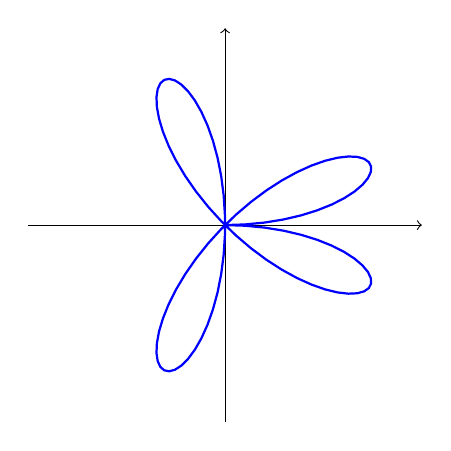
\begin{tikzpicture}
            \draw[->] (-2.5,0)--(2.5,0);
            \draw[->] (0,-2.5)--(0,2.5);
            \draw[line width =0.8pt,blue,domain=0:180,samples=100] plot (\x:{2*sin(\x*4)});
        \end{tikzpicture}
        \ \ \ \ 
        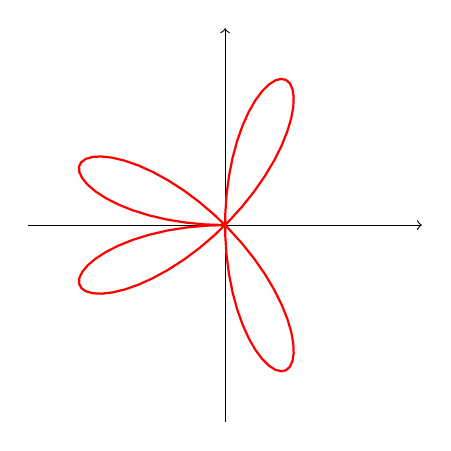
\begin{tikzpicture}
            \draw[->] (-2.5,0)--(2.5,0);
            \draw[->] (0,-2.5)--(0,2.5);
            \draw[line width =0.8pt,red,domain=180:360,samples=100] plot (\x:{2*sin(\x*4)});
        \end{tikzpicture}
    \end{center}
    可以注意到这时有
    $$r(\theta+\pi)=\sin\left(n\theta+n\pi\right)=\sin{n\theta}=r(\theta)$$
    极角相差$\pi$,极径取值相同,因此$\theta\in\left[\dfrac{k\pi}{n},\dfrac{(k+1)\pi}{n}\right]$和$\theta\in\left[\dfrac{k\pi}{n}+\pi,\dfrac{(k+1)\pi}{n}+\pi\right]$对应的两片叶并不会重合.
    所以当$n$为偶数时,$r=\sin(n\theta)$共有$2n$片叶,直接从$0$积分到$2\pi$计算面积也是可行的.
\end{analyze}
\begin{solution}[Solution]
    观察可得该曲线由三个相同的部分组成.于是
    $$\begin{aligned}
        S
        &= 3\cdot\dfrac{1}{2}\int_{0}^{\frac{\pi}{3}}\sin(3\theta)\di\theta \\
        &= 3\cdot\dfrac{1}{6}\left.\left(\dfrac{\varphi}{2}-\dfrac{\sin2\varphi}{4}\right)\right|_0^{\pi} \\
        &= \dfrac{\pi}{4}
    \end{aligned}$$
\end{solution}\noindent
我们再来看一道真题.
\begin{problem}[Problem 2(2021Fall PKU高等数学B期中考试)]
    设奇数$n\geqslant3$,求极坐标系$(r,\theta)$中曲线$r=\sin(n\theta),0\leqslant\theta\leqslant2\pi$围成的封闭图形的面积.
\end{problem}
\begin{solution}[Solution.]
    用平面下极坐标公式可得
    $$S=2n\cdot\dfrac{1}{2}\int_{0}^{\frac{\pi}{2n}}\sin^2(n\theta)\di\theta=\int_{0}^{\frac{\pi}{2}}\sin\varphi\di\varphi=\left.\left(\dfrac{\varphi}{2}-\dfrac{\sin2\varphi}{4}\right)\right|_0^{\frac{\pi}{2}}=\dfrac{\pi}{4}$$
    该方法是计算了每个叶子面积的一半后乘以$2n$而得到总面积.
\end{solution}
\end{document}